\documentclass[12pt, titlepage]{article}
\usepackage[czech]{babel}
\usepackage[IL2]{fontenc}
\usepackage{times}
\usepackage{graphicx}
\usepackage{url}
\usepackage[a4paper, total={17cm, 24cm}, top=3cm, left=2cm]{geometry}
\setcounter{tocdepth}{5} % for showing subsections in TOC

\graphicspath{{./images/}}

\begin{document}
\urlstyle{rm}
% User defined title page
\begin{titlepage}
    \begin{center}
        \textsc{\Huge{Vysoké Učení Technické v Brně\\[0.3em]}}
        \textsc{\huge{Fakulta Informačních Technologií}}
        
        \vspace{\stretch{0.382}}
        
        \LARGE{Tvorba uživatelských rozhraní\\}
        \Huge{Semestrální projekt}
        
        \vspace{\stretch{0.618}}
    \end{center}
    {\Large \phantom{} \hfill \textbf{Lukáš Hais} (xhaisl00)\\
		\phantom{} \hfill \textbf{Tadeáš Kachyňa} (xkachy00)\\
		\today \hfill \textbf{Lukáš Neupauer} (xneupa01)}
\end{titlepage}

\tableofcontents
\newpage

\section{Analýzy a návrhy členů týmu}

\subsection{Lukáš Hais}
\subsubsection{Způsob hledání tématu}
Obepisování blízkých přátel s~dotazem, zda nemají nějakou aplikaci u~které by věděli o~nějakých funkčních/grafických nedostatcích. Následně byla 1~
aplikace vybrána dle osobních preferencí.
\subsubsection{Způsob zkoumání uživatele a jeho potřeby}
Sraz s~uživatelem a~sledování jeho využívání aplikace, doptávání~se na~očekávanou funkcionalitu.\\
Uživatel požaduje aplikaci, která mu umožní zaznamenávat data z~různých oblastí (počet uběhnutých kilometrů, objem vypíte vody za den, hodiny strávené učením,  \ldots) a následné zobrazení grafů podle časového období, filtrované pomocí kategorií spravovaných uživatelem.
\subsubsection{Identifikované potíže}
Neintuitivnost samotné aplikace. Chybí kategorie pro položky podle kterých by bylo možné filtrovat. Nepřehlednost zobrazených grafů.
\subsubsection{Návrh nového řešení}
Znovuvytvoření aplikace s~novým, modernějším designem. Přidání chybějících funkcionalit a~implementace stávajících.

\subsection{Tadeáš Kachyňa}
\subsubsection{Způsob hledání tématu}
Oslovení někoho z mých přátel nebo členů rodiny, zda-li používají nějakou aplikaci u které vědí o nějakých funkčních či grafických nedostatcích. Následně byla mnou jedna aplikace vybrána. 
\subsubsection{Způsob zkoumání uživatele a jeho potřeby}
Navštívení vybraného uživatele a sledování jeho každodenní práce s aplikací (konkrétně s aplikací Fitbit App, která slouží pro detailnější zobrazení statistik naměřených wearable zařízením, které je s touto aplikací spárováno pomocí bluetooth). Bylo vypozorováno, že uživatel není zcela spokojen s aktuální aplikací, má několik nedostatků, které by bylo potřeba vyřešit.
\subsubsection{Identifikované potíže}
Používání aplikace je v některých ohledech docela zdlouhavé a neintuitivní. Při vyhledávání aplikací či ciferníků chybí více filtrů podle kterých by si mohl uživatel snadněji vybrat. Při sledování záznamu svého spánku, srdečního tepu atd. by byl potřeba slider, aby uživatel nemusel zdlouhavě naklikávat jednotlivé naměřené časové úseky.  
\subsubsection{Návrh nového řešení}
V případě této aplikace by byl potřeba redesign a přidání některých funkcí. 

\subsection{Lukáš Neupauer}
\subsubsection{Spôsob hľadania témy}
Pozorovanie okolia a hľadanie zpôsobu zprehľadnenia a väčšieho dosahu informácií. Skúmanie možnosti pridania funkcií do sociálnych médií.

\subsubsection{Spôsob skúmania užívateľa a jepo potreby}
Oslovenie potencionálnych užívateľov a zisťovanie nedostatkov a možností vylepšení aplikácií v ich každodennom používaní. Najčastejšie Discord, Facebook, WhatsApp a Instagram. 

\subsubsection{Identifikované nedostatky}
Neprehľadnosť alebo úplne absencia udalostí v okolí. Užívateľ si pri Facebooku nemôže filtrovať udolosti podľa kategórií a väčšina užívateľ túto vymoženosť ani nevužíva pre komplikovanosť platformy. Pri ostaných táto platformách bola pozorovaná absencia tejto funkcionaloty. 

\subsubsection{Návrh nového riešenia}
Vytvorenie jednoduchej platformy s udalosťami v okolí, s možnosťou zoradienia do kategórií, funciou zobrazenia udalosti iba určitým ľudom (napr. system prateľov) a ďalšími funkciami, ktorá bude slúžiť výužívaná, iba na zvýšenie povedomia a sprehľadnenie udalostí v okolí. 



\newpage



\section{Důvod vybrání zvoleného tématu}
Po společném schůzi se tým demokraticky rozhodl pro volbu aplikace od \emph{Lukáše Haise.} Důvodem k~tomuto kroku bylo celkové zalíbení členů pro daný projekt.

\section{Analýza uživatele}
Uživatel pracuje jakožto číšník a ve volném čase sportuje. Má rád data a~výstupy z~nich, které mu mohou dát nějaký retrospektivní pohled na různé části jeho života. 

\section{Potřeby uživatele}
Uživatel chce využívat aplikaci pro zaznamenávání dat a~následné retrospektivní vyhodnocování zaznamenaných dat.\\
Může jít např. o~sledování četnosti výskytu zlozvyků, udržování nastavených pravidel (např. denní příjem vody), sledování zlepšení fyzických výkonů, \uv{RPG statistiky} při dlouhodobém využívaní aplikace a~zaznamenávání velkého množství dat.

\section{Popis současného řešení}
Uživatel využívá aplikaci \emph{Track and Graph} [obrázek \ref{fig:track-app}] (ke stažení zde: \url{https://f-droid.org/en/packages/com.samco.trackandgraph/}).
\begin{figure}[h]
	\centering
    	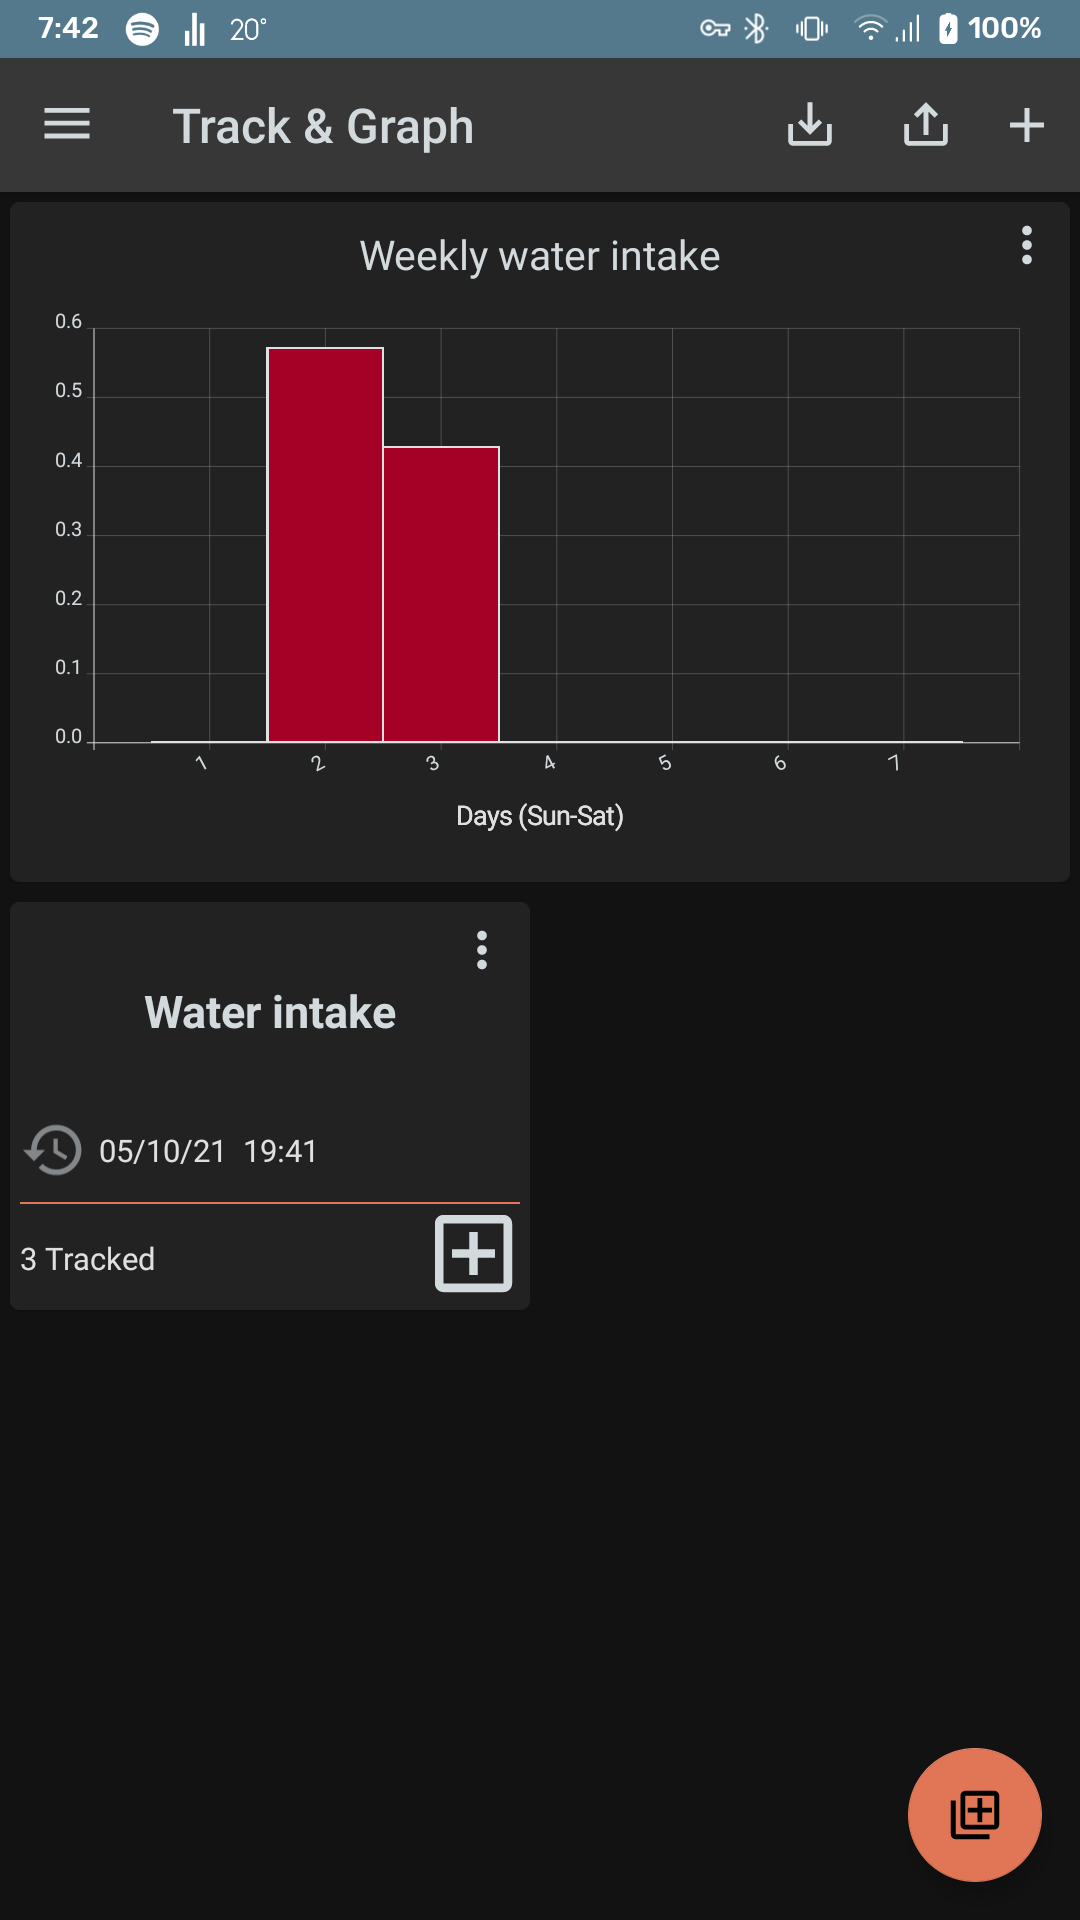
\includegraphics[scale=0.15]{trackgraph-pic}
    \caption{\emph{Track and Graph} aplikace}
    \label{fig:track-app}
\end{figure}



\section{Návrh zadání}
V našem případě půjde o~znovuvytvoření již existující aplikace, modernizaci designu a~přidání chybějících funkcionalit.
\subsection{Funkcionalita}
Přidání kategorií pro lepší filtraci při vytváření grafů. Kategorie budou mít vlastní měrné jednotky (např. litry pro vypité pití) a další volitelné parametry.\\
Toto by mělo směrovat k~lepším výstupům samotné aplikace a~tudíž k většímu zájmu o~používání aplikace.
\subsection{Grafika}
Modernizace stávající grafiky. Vytvoření menu ve kterém lze přidávat položky do databáze, či zobrazování grafů (které mohou být členěny do skupin).


\section{Návrh řešení}
TO-DO

\end{document}
